\documentclass[11pt,a4paper]{article}

\usepackage[utf8]{inputenc}
\usepackage[T1]{fontenc}
\usepackage{lmodern}
\usepackage{geometry}
\usepackage{hyperref}
\usepackage{enumitem}
\usepackage{amsmath,amssymb}
\usepackage{graphicx}
\usepackage{xcolor}
\usepackage{tikz}

\geometry{margin=2.5cm}

\title{VeriScript: A Protocol for Script Attestation on Cardano}
\author{%
  VeriScript Project \\
  \small{Mark Petruska <mark.petruska@protonmail.com>, Adam Valach <avalach84@gmail.com>}
}
\date{\today}

\hypersetup{
    colorlinks,
    citecolor=black,
    filecolor=black,
    linkcolor=black,
    urlcolor=black
}

\usetikzlibrary{shapes, arrows, positioning}

\tikzset{
  inputnode/.style={draw, rounded rectangle, minimum width=2.5cm, minimum height=1cm, align=center, fill=red!20},
  outputnode/.style={draw, rounded rectangle, minimum width=2.5cm, minimum height=1cm, align=center, fill=green!20},
  processnode/.style={draw, rectangle, minimum width=3cm, minimum height=1cm, align=center, fill=blue!20},
  mintingpolicynode/.style={draw, tape, aspect=2, minimum width=3cm, minimum height=1cm, align=center, fill=orange!20},
  arrow/.style={->, thick},
  dashedarrow/.style={->, dashed, thick}
}

\begin{document}

\maketitle

\begin{abstract}
VeriScript is a protocol on the Cardano blockchain that enables users to verify both the source code and the on-chain binaries of scripts they interact with.
It introduces a structured \emph{attestation} mechanism based on native tokens, reference scripts, and script-addressed UTxOs to bind script hashes and addresses to human-readable metadata and signed claims from recognizable authors.
\end{abstract}

\setcounter{tocdepth}{2}
\tableofcontents

\section{Introduction}

Smart-contract users on Cardano often interact with script addresses or policy IDs whose provenance and implementation details are opaque, making security reviews and trust assessments difficult.%
\footnote{Scripts on Cardano are associated with UTxOs at script addresses in the extended UTxO (EUTxO) model, and can be referenced via hashes or policy IDs.\,\cite{cardano-eutxo}}
VeriScript provides an on-chain attestation layer that lets authors and reviewers publicly link script binaries and identifiers to auditable source code and descriptive metadata.

The protocol defines:
\begin{itemize}[noitemsep]
  \item \textbf{Author tokens}, which identify attestation signers.
  \item \textbf{Attestation UTxOs}, script-addressed outputs that hold reference scripts, structured metadata, and non-reusable signature tokens.
  \item \textbf{Signature tokens}, which represent individual signers' endorsements of a particular attestation.
\end{itemize}

\section{Design Goals}

The main design goals of VeriScript are:
\begin{itemize}[noitemsep]
  \item \textbf{Verifiable provenance:} Bind a script hash/address/policy ID to a specific source-code revision (e.g.\ a GitHub commit) and minimal description.
  \item \textbf{Signer accountability:} Associate attestations with signers represented by author tokens controlled via minting policies.
  \item \textbf{Composability with Cardano primitives:} Use standard Cardano features such as native tokens, minting policies, script addresses, and reference scripts without protocol-level changes.\,\cite{cardano-eutxo}\cite{cip33}\cite{minting-nfts}
  \item \textbf{Low overhead and reusability:} Allow multiple signers to attest to the same script via a shared attestation UTxO and non-reusable signature tokens, while respecting minimum ADA requirements.\,\cite{min-ada}
  \item \textbf{Reclaimability:} Enable the original author to retire obsolete attestations and reclaim locked ADA by burning associated signature tokens.
\end{itemize}

\section{System Model and Roles}

\subsection{Blockchain Environment}

VeriScript is deployed on the Cardano blockchain, which uses an extended UTxO model.%
\footnote{Cardano UTxOs can be addressed by public keys or scripts, and may carry inline datums or reference scripts.\,\cite{cardano-eutxo}\cite{cip33}}
Transactions consume existing UTxOs and create new ones, optionally involving Plutus scripts, minting policies, and reference scripts.\,\cite{cardano-eutxo}\cite{cip33}

The protocol assumes:
\begin{itemize}[noitemsep]
  \item Native tokens and minting policies as defined in the Cardano ledger.\,\cite{minting-nfts}
  \item Reference scripts and reference inputs per CIP-31 and CIP-33 to store scripts on-chain in UTxOs.\,\cite{cip31}\cite{cip33}
  \item Minimum ADA requirements based on UTxO size and asset content.\,\cite{min-ada}
\end{itemize}

\subsection{Actors}

\paragraph{Signer.}
An entity capable of:
\begin{itemize}[noitemsep]
  \item Minting and controlling a unique \emph{author token}.
  \item Building and submitting Cardano transactions that create attestation UTxOs or add their minted unique \emph{signature tokens}.
  \item Verifying script source, compilation and derived identifiers off-chain.
\end{itemize}

\paragraph{User (Verifier).}
An entity that queries the VeriScript index/backend or directly the chain to find attestation UTxOs associated with specific scripts, then decides whether to trust them based on signers and statistics.

\paragraph{Backend / Indexer.}
Off-chain infrastructure that:
\begin{itemize}[noitemsep]
  \item Indexes attestation UTxOs and associated tokens.
  \item Exposes query interfaces based on script hash, address, policy IDs, or signer identity.
  \item Computes statistics (e.g.\ number of signers, signer reputation) to support trust decisions.
\end{itemize}

\section{On-chain Objects}

\subsection{Author Token}

An \emph{author token} is a native asset minted under a dedicated minting policy that uniquely identifies a signer.
The intended semantics are:
\begin{itemize}[noitemsep]
  \item One author token per signer (or signer identity), typically implemented as an NFT.\break\cite{minting-nfts}
  \item The minting policy enforces that a token can be minted only once.
  \item The token policy ID is used to verify ownership when minting signature tokens.
  \item The token implementation is similar to a CIP-68 token holding metadata that can potentially be used to link this digital identity to a real world one (if it is the choice of the signer).\,\cite{cip68}
\end{itemize}

The author token serves as a capability: possession of it is required to mint signature tokens that represent attestations issued by the corresponding signer.

\subsection{Signature Token}

A \emph{signature token} is a native token that represents one signer's endorsement of a specific attestation.
It is minted under a \emph{signature minting policy} which enforces:
\begin{itemize}[noitemsep]
  \item \textbf{Ownership check:} Minting a signature token requires demonstrating control of the associated author token.
        This can be enforced by requiring the author token to be moved in the same transaction, for example by sending it from the signer to themself.
  \item \textbf{Burnability:} Signature tokens can be burned under the same policy, allowing the original author of the UTxO or the original signer to burn the signature token.
\end{itemize}

\subsection{Attestation Script and UTxO}

VeriScript defines an \emph{attestation script} whose address holds \emph{attestation UTxOs}.
Each attestation UTxO has the following structure:
\begin{itemize}[noitemsep]
  \item \textbf{Address:} The UTxO resides at the attestation script address.
  \item \textbf{Value:}
    \begin{itemize}[noitemsep]
      \item At least a protocol-compliant minimum amount of ADA, configured so that the UTxO can host multiple signature tokens without additional top-ups (e.g.\ $\geq 4$ ADA, subject to actual min-ADA rules).\,\cite{cardano-eutxo}\cite{min-ada}
      \item At least one signature tokens from various signers. The number of tokens a single UTxO can hold must be maximized to avoid the possibility of creating unspendable outputs.
    \end{itemize}
  \item \textbf{Datum:} An \emph{attestation datum} containing structured information that the signers attest to.
  \item \textbf{Reference script:} The actual script binary attached as a reference script per CIP-33.\,\cite{cip33}
\end{itemize}

The attestation script enforces the allowed state transitions, including:
\begin{itemize}[noitemsep]
  \item Creation of new attestation UTxOs from arbitrary inputs.
  \item Addition of signature tokens to existing attestation UTxOs without changing the attestation datum.
  \item Spending and retirement of attestation UTxOs under controlled conditions (original author and signer only).
\end{itemize}

\subsection{Attestation Datum}

The \emph{attestation datum} is an immutable record of what is being attested.
It includes at least:
\begin{itemize}[noitemsep]
  \item A GitHub (or equivalent) reference including a repository locator and a specific commit hash, pointing to the source code.
  \item A minimal human-readable description of the script to help identification.
  \item The script hash of the compiled on-chain script.
  \item The script address, if applicable.
  \item The staking policy ID, if applicable.
  \item The minting policy ID, if applicable.
  \item The signer token name of the original author.
\end{itemize}

All signers that add signature tokens to the same attestation UTxO agree on the contents of this datum.

\section{Protocol Workflows}

\subsection{Signer Setup: Author Token Creation}

This setup is performed once per signer identity:

\begin{enumerate}[noitemsep]
  \item The signer constructs a transaction that:
    \begin{itemize}[noitemsep]
      \item Mints exactly one author token under this policy.
      \item Creates the corresponding "datum metadata" similarly to CIP-68.\cite{cip68}
      \item Sends the author token to an address controlled by the signer.
    \end{itemize}
  \item The transaction is submitted and included on-chain, finalizing the creation of the author token.
\end{enumerate}

After this phase, the signer holds their author token and can participate in VeriScript attestations.

\subsubsection{Transaction diagram}

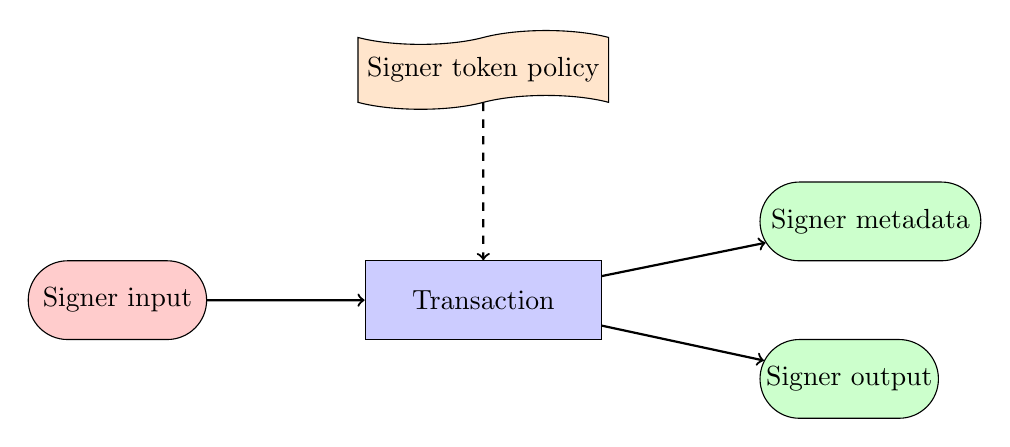
\begin{tikzpicture}[node distance=2cm]

% Nodes
\node[inputnode] (I1) {Signer input};
\node[processnode, right=of I1] (TX) {Transaction};
\node[mintingpolicynode, above=of TX] (MP) {Signer token policy};
\node[outputnode, right=of TX, yshift=1cm] (O1) {Signer metadata};
\node[outputnode, right=of TX, yshift=-1cm] (O2) {Signer output};

% Edges
\draw[arrow] (I1) -- (TX);
\draw[dashedarrow] (MP) -- (TX);
\draw[arrow] (TX) -- (O1);
\draw[arrow] (TX) -- (O2);

\end{tikzpicture}

Where:
\begin{itemize}
  \item \textbf{Signer input}: an input UTxO from the signer's wallet, covers the transaction fee and used in signer token name creation to ensure that  the same name cannot be generated.
  \item \textbf{Signer token policy}: the minting policy that governs the minting and burning of the \textit{signer token}s.
  \item \textbf{Signer metadata}: an UTxO stored at the address of the \textit{signer metadata} script address, stores optional information about the signer.
  \item \textbf{Signer output}: an UTxO send back to the signer's wallet, contains the minted \textit{signer token}.
\end{itemize}


\subsection{Signer Attestation Creation (New Attestation)}

When no suitable attestation UTxO exists for a script, the signer creates a new one:

\begin{enumerate}[noitemsep]
  \item The signer obtains the script source code to be attested (e.g.\ by cloning a Git repository at a chosen commit).
  \item The signer compiles the source code using the intended toolchain, deriving:
    \begin{itemize}[noitemsep]
      \item The script binary (e.g.\ flat or CBOR-encoded Plutus script).
      \item The script hash.
      \item The script address, if the script is used as a spending script.
      \item The staking policy ID, if relevant.
      \item The minting policy ID, if relevant.
    \end{itemize}
  \item The signer constructs an \emph{attestation datum} containing:
    \begin{itemize}[noitemsep]
      \item The GitHub (or equivalent) repository and commit hash.
      \item A minimal description of the script.
      \item The script hash and any applicable script address or policy IDs.
      \item Including his own author token's name
    \end{itemize}
  \item The signer builds a transaction that:
    \begin{itemize}[noitemsep]
      \item Creates a new UTxO at the attestation script address, with:
            \begin{itemize}[noitemsep]
              \item The attestation datum.
              \item Sufficient ADA (e.g.\ 4 ADA, tuned to min-UTxO rules for a reference script plus future signature tokens).\,\cite{cardano-eutxo}\cite{min-ada}
              \item One newly minted signature token under the signature minting policy.
            \end{itemize}
      \item Attaches the script binary as a reference script on this new UTxO.\,\cite{cardano-eutxo}
      \item Demonstrates control of the author token, as required by the signature minting policy.
            This can be implemented by moving the author token in the transaction, for example sending it back to the signer’s own address under specific constraints.
    \end{itemize}
  \item The transaction is submitted and finalized, creating a new attestation UTxO with the signer’s initial signature token.
\end{enumerate}

The resulting attestation UTxO serves as a canonical on-chain reference for that script, linking source, binary, and identifiers.

\subsubsection{Transaction diagram}

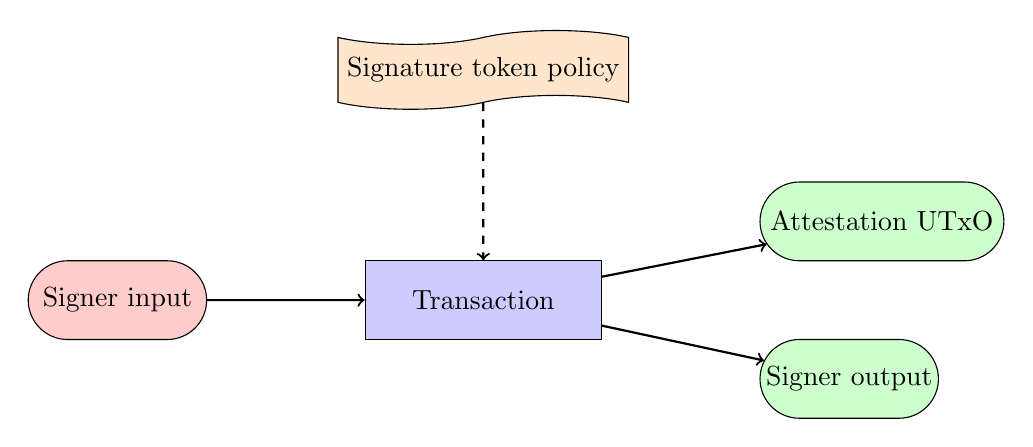
\begin{tikzpicture}[node distance=2cm]

% Nodes
\node[processnode] (TX) {Transaction};
\node[inputnode, left=of TX] (I1) {Signer input};
\node[mintingpolicynode, above=of TX] (MP) {Signature token policy};
\node[outputnode, right=of TX, yshift=1cm] (O1) {Attestation UTxO};
\node[outputnode, right=of TX, yshift=-1cm] (O2) {Signer output};

% Edges
\draw[arrow] (I1) -- (TX);
\draw[dashedarrow] (MP) -- (TX);
\draw[arrow] (TX) -- (O1);
\draw[arrow] (TX) -- (O2);

\end{tikzpicture}

Where:
\begin{itemize}
  \item \textbf{Signer input}: an input UTxO from the signer's wallet that contains the \textit{signer token}.
  \item \textbf{Signature token policy}: the minting policy that governs the minting and burning of the \textit{signature tokens}.
  \item \textbf{Attestation UTxO}: an UTxO stored at the address of the \textit{attestation holder} script address, stores the \textit{attestation datum} described above. Contains the minted \textit{signature token}.
  \item \textbf{Signer output}: an UTxO send back to the signer's wallet, contains the validated \textit{signer token}.
\end{itemize}


\subsection{Signer Attestation on Existing UTxO}

If an attestation UTxO already exists for the target script, a signer can add their endorsement:

\begin{enumerate}[noitemsep]
  \item The signer locates the existing attestation UTxO via the VeriScript frontend/backend.
  \item The signer independently:
    \begin{itemize}[noitemsep]
      \item Downloads the referenced source code (e.g.\ from the GitHub commit in the datum).
      \item Recompiles and verifies that the resulting script hash, address, and policy IDs match the attestation datum.
    \end{itemize}
  \item If the attestation datum is correct, the signer constructs a transaction that:
    \begin{itemize}[noitemsep]
      \item Consumes the existing attestation UTxO.
      \item Creates a new attestation UTxO with:
            \begin{itemize}[noitemsep]
              \item The \emph{same} attestation datum.
              \item The original ADA and signature tokens.
              \item An additional signature token minted under the signature minting policy for this signer.
            \end{itemize}
      \item Proves control of the signer's author token as required by the signature minting policy.
    \end{itemize}
  \item The transaction is submitted and, upon inclusion, the attestation UTxO now reflects the extra signature token.
\end{enumerate}

If the signer disagrees with the datum (e.g.\ the source does not reproduce the script hash), they instead create a new attestation UTxO as in the previous subsection, with corrected data.

\subsubsection{Transaction diagram}

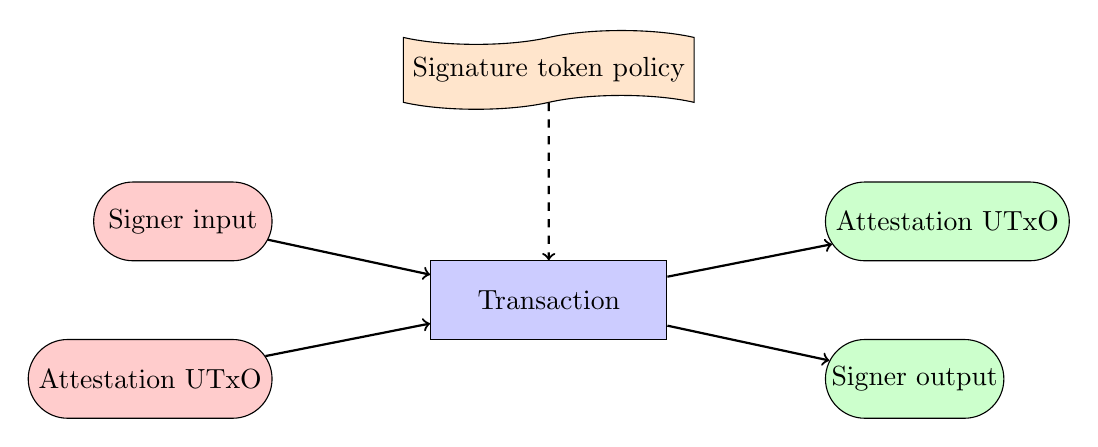
\begin{tikzpicture}[node distance=2cm]

% Nodes
\node[processnode] (TX) {Transaction};
\node[mintingpolicynode, above=of TX] (MP) {Signature token policy};
\node[inputnode, left=of TX, yshift=1cm] (I1) {Signer input};
\node[inputnode, left=of TX, yshift=-1cm] (I2) {Attestation UTxO};
\node[outputnode, right=of TX, yshift=1cm] (O1) {Attestation UTxO};
\node[outputnode, right=of TX, yshift=-1cm] (O2) {Signer output};

% Connections
\draw[arrow] (I1) -- (TX);
\draw[arrow] (I2) -- (TX);
\draw[dashedarrow] (MP) -- (TX);
\draw[arrow] (TX) -- (O1);
\draw[arrow] (TX) -- (O2);

\end{tikzpicture}

Where:
\begin{itemize}
  \item \textbf{Signer input}: an input UTxO from the signer's wallet that contains the \textit{signer token}.
  \item \textbf{Signature token policy}: the minting policy that governs the minting and burning of the \textit{signature tokens}.
  \item \textbf{Attestation UTxO} input: the UTxO that will be signed.
  \item \textbf{Attestation UTxO} output: the "new" \textit{attestation UTxO} that has the same values as the original with the newly minted \textit{signature token} attached.
  \item \textbf{Signer output}: an UTxO send back to the signer's wallet, contains the validated \textit{signer token}.
\end{itemize}


\subsection{User Verification Journey}

A user who wants to verify a script performs:

\begin{enumerate}[noitemsep]
  \item The user queries the VeriScript backend (e.g. through the frontend application) or an indexer with a script hash, script address, staking policy ID, or minting policy ID to retrieve all relevant attestation UTxOs.
  \item For each candidate attestation UTxO, the user can inspect:
    \begin{itemize}[noitemsep]
      \item The attestation datum (source reference, commit hash, description, script hash, addresses, and policies).
      \item The set and count of signature tokens, each identifying a signer via its minting policy and token name.
      \item Optional off-chain metadata or reputation scores about signers.
    \end{itemize}
  \item The user forms a trust decision based on:
    \begin{itemize}[noitemsep]
      \item The number and reputability of signers who have attested to this datum.
      \item Any discrepancies across multiple attestation UTxOs referring to the same script identifiers.
      \item Other statistics provided by the VeriScript frontend (e.g. specific authors attestation numbers, counter-attested UTxOs, etc)
    \end{itemize}
\end{enumerate}

Users can, but are not required to, locally rebuild the script from the referenced source to further increase assurance.


\subsection{Attestation Retirement}

When an attestation UTxO is no longer needed (e.g.\ script deprecated or migrated), the original author may retire it:

\begin{enumerate}[noitemsep]
  \item The attestation script enforces a rule that allows the creator to spend the attestation UTxO.
  \item The original author constructs a transaction that:
    \begin{itemize}[noitemsep]
      \item Consumes the attestation UTxO.
      \item Burns all associated signature tokens under the signature minting policy.
      \item Returns the locked ADA to an address of their choice.
    \end{itemize}
  \item Once the transaction is finalized, the attestation is effectively removed and the ADA is reclaimed.
\end{enumerate}

\subsubsection{Transaction diagram}

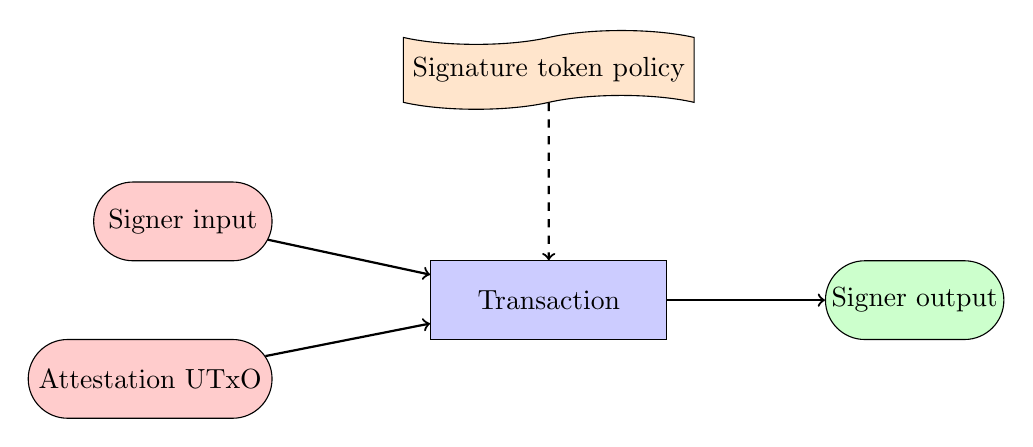
\begin{tikzpicture}[node distance=2cm]

% Nodes
\node[processnode] (TX) {Transaction};
\node[mintingpolicynode, above=of TX] (MP) {Signature token policy};
\node[inputnode, left=of TX, yshift=1cm] (I1) {Signer input};
\node[inputnode, left=of TX, yshift=-1cm] (I2) {Attestation UTxO};
\node[outputnode, right=of TX] (O1) {Signer output};

% Connections
\draw[arrow] (I1) -- (TX);
\draw[arrow] (I2) -- (TX);
\draw[dashedarrow] (MP) -- (TX);
\draw[arrow] (TX) -- (O1);

\end{tikzpicture}

Where:
\begin{itemize}
  \item \textbf{Signer input}: an input UTxO from the signer's wallet that contains the \textit{signer token}.
  \item \textbf{Signature token policy}: the minting policy that governs the minting and burning of the \textit{signature tokens}.
  \item \textbf{Attestation UTxO}: the retiring \textit{attestation UTxO}, all the signature tokens it contains must be burned.
  \item \textbf{Signer output}: an UTxO send back to the signer's wallet, contains the validated \textit{signer token}.
\end{itemize}


\section{Script and Policy Design}

\subsection{Attestation Script Logic}

At a high level, the attestation validator should enforce:

\begin{itemize}[noitemsep]
  \item \textbf{Datum immutability for additions:} When an attestation UTxO is spent and recreated to add signature tokens, the output datum must equal the input datum.
  \item \textbf{Controlled retirement:} Spending that changes or removes the datum (i.e.\ not a simple signature-token addition) must satisfy additional constraints (e.g.\ possession of an author-control token).
  \item \textbf{Conservation of ADA and tokens:} Apart from explicit burns under minting policies, the ADA and existing signature tokens should be preserved when adding new signatures.
\end{itemize}

This logic can be implemented in a Plutus script that inspects:
\begin{itemize}[noitemsep]
  \item The input and output UTxOs at the attestation address.
  \item The datums and token bundles of those UTxOs.
  \item Redeemer fields specifying the intended action (e.g.\ ``AddSignature'' vs.\ ``Retire'').
\end{itemize}

\subsection{Author Token Minting Policy}

The author token minting policy should:
\begin{itemize}[noitemsep]
  \item Enforce that a unique token is minted for each author.
  \item Require the creation of a metadata (similar to CIP-68) during the minting operation.
\end{itemize}

\subsection{Signature Token Minting Policy}

The signature minting policy should:
\begin{itemize}[noitemsep]
  \item Require that the transaction demonstrates ownership of the corresponding author token by requiring the author token to appear as an input.
  \item Permit burning of existing signature tokens, in case the signer reconsiders his stance on an attestation or if the original author retires the attestation UTxO.
\end{itemize}

\section{Incentives and Security Considerations}

\subsection{Incentive Structure}

The primary incentive for signers is community benefit and reputational gain:
\begin{itemize}[noitemsep]
  \item Security auditors and experts can publicly attest to scripts, building a verifiable record of their reviews.
  \item Script authors can publish attestations for their own contracts, improving discoverability and transparency.
  \item DApp users can rely on aggregated attestations and signer reputations to inform interaction decisions.
\end{itemize}

Signers pay transaction fees and lock some ADA in attestation UTxOs, but can share UTxOs and reclaim ADA upon retirement.

\subsection{Threat Model and Mitigations}

Potential threats include:
\begin{itemize}[noitemsep]
  \item \textbf{Malicious or incompetent signers:} A signer may attest to incorrect or malicious scripts.
        Mitigation: rely on multiple independent signers, public reputation, and optional local verification of source and binaries.
  \item \textbf{Data inconsistency:} Different attestations might claim conflicting information about a script.
        Mitigation: users and backends can compare datums and highlight inconsistencies; signers can create corrected attestations when needed.
  \item \textbf{UTxO bloat:} Large reference scripts and many attestations could increase UTxO set size.
        Mitigation: limit the number of singature tokens that can be put on the same UTxO.
  \item \textbf{Author token compromise:} If a signer's key or author token is compromised, an attacker can mint fraudulent signature tokens.
        Mitigation: public announcements and possibly specific warnings appearing on the VeriScript frontend application.
\end{itemize}

\section{Implementation Considerations}

\subsection{Reference Scripts and Min-ADA}

Attestation UTxOs store the script binary as a reference script, allowing subsequent transactions to use the script without re-attaching it in the witness set, improving throughput and reducing fees.\,\cite{cardano-eutxo}\cite{cip31}\cite{cip33}
Because reference scripts increase UTxO size, the minimum ADA requirement grows with script and token-bundle size, so the protocol recommends allocating generous ADA (e.g.\ 4 ADA) to accommodate multiple signatures over time.\,\cite{min-ada}

\subsection{Off-chain Infrastructure}

A typical deployment includes:
\begin{itemize}[noitemsep]
  \item A backend indexer tracking:
        \begin{itemize}[noitemsep]
          \item All UTxOs at the attestation script address.
          \item Their datums, reference scripts, and native tokens.
        \end{itemize}
  \item APIs for:
        \begin{itemize}[noitemsep]
          \item Querying by script hash, address, policy ID, or signer.
          \item Computing statistics such as number of attestations and distinct signers.
        \end{itemize}
  \item Optional integration with GitHub or other hosting platforms to validate repository URLs and commit hashes.
\end{itemize}

\subsection{Extensibility}

Future extensions may include:
\begin{itemize}[noitemsep]
  \item Versioned attestation schemas enabling richer metadata (e.g.\ build instructions, dependencies).
  \item Support for non-Git platforms or content-addressed storage (e.g.\ IPFS).
  \item Reputation systems or staking mechanisms for signers.
  \item Formal verification artifacts (e.g.\ references to proofs) attached in the datum or via additional reference UTxOs.
\end{itemize}

\section{Conclusion}

VeriScript defines an on-chain attestation protocol for Cardano that links script binaries and identifiers to reproducible source-code references, while recording endorsements from identifiable signers.
By combining author tokens, signature tokens, attestation UTxOs, and reference scripts, it enables transparent and composable provenance tracking for smart contracts and policies, without requiring changes to the underlying ledger.

\bibliographystyle{plain}
\begin{thebibliography}{9}

\bibitem[CIP-31]{cip31}
Cardano Improvement Proposal 31: Reference Inputs (CIP-31). \url{https://cips.cardano.org/cip/CIP-31}.

\bibitem[CIP-33]{cip33}
Cardano Improvement Proposal 33: Reference Scripts (CIP-33). \url{https://cips.cardano.org/cip/CIP-33}.

\bibitem[CIP-68]{cip68}
Cardano Improvement Proposal 33: Datum Metadata Standard (CIP-68). \url{https://cips.cardano.org/cip/CIP-68}.

\bibitem[EUTxO]{cardano-eutxo}
Scripts and the Extended UTXO Model. Cardano / Plutus documentation. \url{https://plutus.cardano.intersectmbo.org/docs/essential-concepts/eutxo}.

\bibitem[Min-Ada]{min-ada}
Minimum ADA Value Requirement. Cardano Ledger documentation. \url{https://cardano-ledger.readthedocs.io/en/latest/explanations/min-utxo-mary.html}.

\bibitem[Minting]{minting-nfts}
Minting NFTs on Cardano. Cardano Developer Portal. \url{https://developers.cardano.org/docs/native-tokens/minting-nfts/}.

\end{thebibliography}

\end{document}
